% --------------------------------------------------------------
% This is all preamble stuff that you don't have to worry about.
% Head down to where it says "Start here"
% --------------------------------------------------------------
 
\documentclass[12pt]{article}
 
\usepackage[margin=1in]{geometry} 
\usepackage{amsmath,amsthm,amssymb}
\usepackage{tikz}
 
\newcommand{\N}{\mathbb{N}}
\newcommand{\Z}{\mathbb{Z}}
 
\newenvironment{theorem}[2][Theorem]{\begin{trivlist}
\item[\hskip \labelsep {\bfseries #1}\hskip \labelsep {\bfseries #2.}]}{\end{trivlist}}
\newenvironment{lemma}[2][Lemma]{\begin{trivlist}
\item[\hskip \labelsep {\bfseries #1}\hskip \labelsep {\bfseries #2.}]}{\end{trivlist}}
\newenvironment{exercise}[2][Exercise]{\begin{trivlist}
\item[\hskip \labelsep {\bfseries #1}\hskip \labelsep {\bfseries #2.}]}{\end{trivlist}}
\newenvironment{question}[2][Question]{\begin{trivlist}
\item[\hskip \labelsep {\bfseries #1}\hskip \labelsep {\bfseries #2.}]}{\end{trivlist}}
\newenvironment{proposition}[2][Proposition]{\begin{trivlist}
\item[\hskip \labelsep {\bfseries #1}\hskip \labelsep {\bfseries #2.}]}{\end{trivlist}}
\newenvironment{corollary}[2][Corollary]{\begin{trivlist}
\item[\hskip \labelsep {\bfseries #1}\hskip \labelsep {\bfseries #2.}]}{\end{trivlist}}
 
\begin{document}
 
% --------------------------------------------------------------
%                         Start here
% --------------------------------------------------------------
 
%\renewcommand{\qedsymbol}{\filledbox}
 
\title{Homework 2}%replace X with the appropriate number
\author{Team F\\ %replace with your name
CSC 565 - Graph Theory} %if necessary, replace with your course title
 
\maketitle
 
\begin{question}{1}
Find a graph G with 5 vertices which has neither a clique of size 3 nor an independent set of size 3.
\end{question}

\begin{align*}
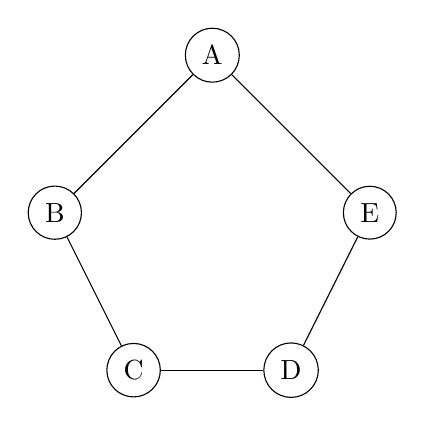
\begin{tikzpicture}
    \node[shape=circle,draw=black] (C) at (1,0) {C};
    \node[shape=circle,draw=black] (B) at (0,2) {B};
    \node[shape=circle,draw=black] (A) at (2,4) {A};
    \node[shape=circle,draw=black] (D) at (3,0) {D};
    \node[shape=circle,draw=black] (E) at (4,2) {E};
    \path [] (A) edge node[left] {} (B);
    \path [] (B) edge node[left] {} (C);
    \path [] (C) edge node[left] {} (D);
    \path [] (D) edge node[left] {} (E);
    \path [] (E) edge node[left] {} (A);
\end{tikzpicture}
\end{align*}


\begin{question}{5}
	Prove or disprove: if $G$ is a disconnected graph, then $\overline{G}$, the complement of $G$, is connected.\\	
	
	i. Let $u$, $v$ be disconnected vertices in $G$. Since there is no $uv$ edge in $G$, there must be a $uv$ edge in $\overline{G}$. Thus $u$ $v$ are connected in $\overline{G}$\\
		
	ii. Let $u$, $v$ be on the same component in $G$. Let $w$ be a vertex on a separate component in $G$. There must be a $uw$ edge in $\overline{G}$. There must also be a $vw$ edge in $\overline{G}$. 
	Because there is a $uw$ path, and a $vw$ path, by Lemma 1.2.5 there must also be a $uv$ path. Thus $u$ and $v$ are connected in $\overline{G}$\\
	
	Because there exists a path between any two vertices in $\overline{G}$ it is a connected graph.
\end{question}

\begin{question}{7}
A graph is called chordal if it has no induced subgraph isomorphic to $C_{n}$ for any $n \leq 4$. Which of the following 10-vertex graphs are chordal?
\end{question}

\begin{align*}	
\end{align*}
 
% --------------------------------------------------------------
%     You don't have to mess with anything below this line.
% --------------------------------------------------------------
 
\end{document}